\subsection{Implementierung API und Datenbank}
Der erste benötigte Dienst für die Webanwendung ist die GraphQL API.
Mit \spverb+amplify add api+ startet der Konfigurationsassistent.
Da die Authentifizierung mit Cognito erst zu einem späteren Zeitpunkt hinzugefügt wird, erfolgt sie so lange mittels API Key.
Die Änderung der Authentifizierung erfolgt im Abschnitt \textit{\ref{ImpAuth} \nameref{ImpAuth}}.
Nach Bestätigung des letzten Schrittes öffnet sich die Datei \verb+schema.graphql+, die das Schema der API darstellt.
In dieser Datei werden alle benötigten Objekttypen erstellt.
\clearpage
\begin{lstlisting}[basicstyle=\ttfamily\small, breaklines=true , frame = single, backgroundcolor=\color{flashwhite} ]
Please select from one of the below mentioned services:(*@ \textrm{GraphQL} @*)
Provide API name:(*@ \textrm{amplify-kumo-api} @*)
Choose the default authorization type for the API:(*@ \textrm{API key} @*)
Enter a description for the API key:(*@ \textrm{My-Dev-ApiKey} @*)
After how many days from now the API key should expire (1-365):(*@ \textrm{7} @*)
Do you want to configure advanced settings for the GraphQL API:(*@ \textrm{No} @*)
Do you have an annotated GraphQL schema?(*@ \textrm{No} @*)
Do you want a guided schema creation?(*@ \textrm{Yes} @*)
What best describes your project:
Single object with fields (e.g., Todo with ID, name, description)
Do you want to edit the schema now?(*@ \textrm{Yes} @*)
\end{lstlisting}

Im Rahmen der Bachelorarbeit wird nur ein Objekttyp mit dem Namen \spverb+Account+ benötigt.
Es werden weiterhin alle verfügbaren Felder angegeben.
Werden in Zukunft neue Felder oder weitere Typen benötigt, kann die Datei \verb+schema.graphql+ jederzeit angepasst werden.
\\
\begin{lstlisting}[basicstyle=\ttfamily\small, breaklines=true , frame = single, backgroundcolor=\color{flashwhite} ]
type Account @model {
  id: ID!
  accountid: String!
  name: String!
  email: String!
  num: Int!
  status: String!
}

\end{lstlisting}

Alle angegeben Felder müssen im späteren Verlauf von der Lambda-Funktion abgerufen und gespeichert werden.
Mit dem Befehl \verb+amplify push+ wird die API in der Cloud bereitgestellt.
Im folgenden Dialog besteht die Möglichkeit alle möglichen Mutationen und Queries generieren zu lassen.
Wie bereits im Abschnitt \textit{\ref{GraphQL} \nameref{GraphQL}} erwähnt, wäre es bei GraphQL normalerweise üblich die Query-Typen etc. manuell zu erzeugen.
AppSync übernimmt hier also wie versprochen einen großen Teil der Arbeit.
\\
\begin{lstlisting}[basicstyle=\ttfamily\small, breaklines=true , frame = single, backgroundcolor=\color{flashwhite} ]

# You will be walked through the following questions for GraphQL code generation

Do you want to generate code for your newly created GraphQL API? (*@ \textrm{Y} @*)
Choose the code generation language target:(*@ \textrm{javascript} @*)

Do you want to generate/update all possible GraphQL operations -
queries, mutations and subscriptions? (*@ \textrm{Y} @*)

\end{lstlisting}


Sobald der Prozess fertig gestellt ist, sind die Dienste AWS AppSync und DynamoDB konfiguriert.
Dank DynamoDB-Resolver wurde eine entsprechende DynamoDB-Tabelle angelegt und konfiguriert.
In der Webkonsole von AWS kann überprüft werden, ob der Vorgang erfolgreich war.
Die Ansicht von AppSync zeigt im Menüpunkt \grqq Data Sources\grqq{}, dass eine DynamoDB-Tabelle passend zum GraphQL Objekttyp erstellt wurde.
Der Name der Tabelle wurde nach dem GraphQL Objekttyp gewählt.
Nun ist es möglich per API auf die Datenbank zuzugreifen und Daten abzufragen.
Die jeweilige Abfrage findet im Abschnitt \textit{\ref{ReactFrontend} \nameref{ReactFrontend}} statt.
Bevor das Frontend jedoch Anfragen an die Datenbank ausführen kann, muss Lambda konfiguriert werden, sodass Daten gespeichert werden.
\\
\begin{figure}[htbp]
    \centering
    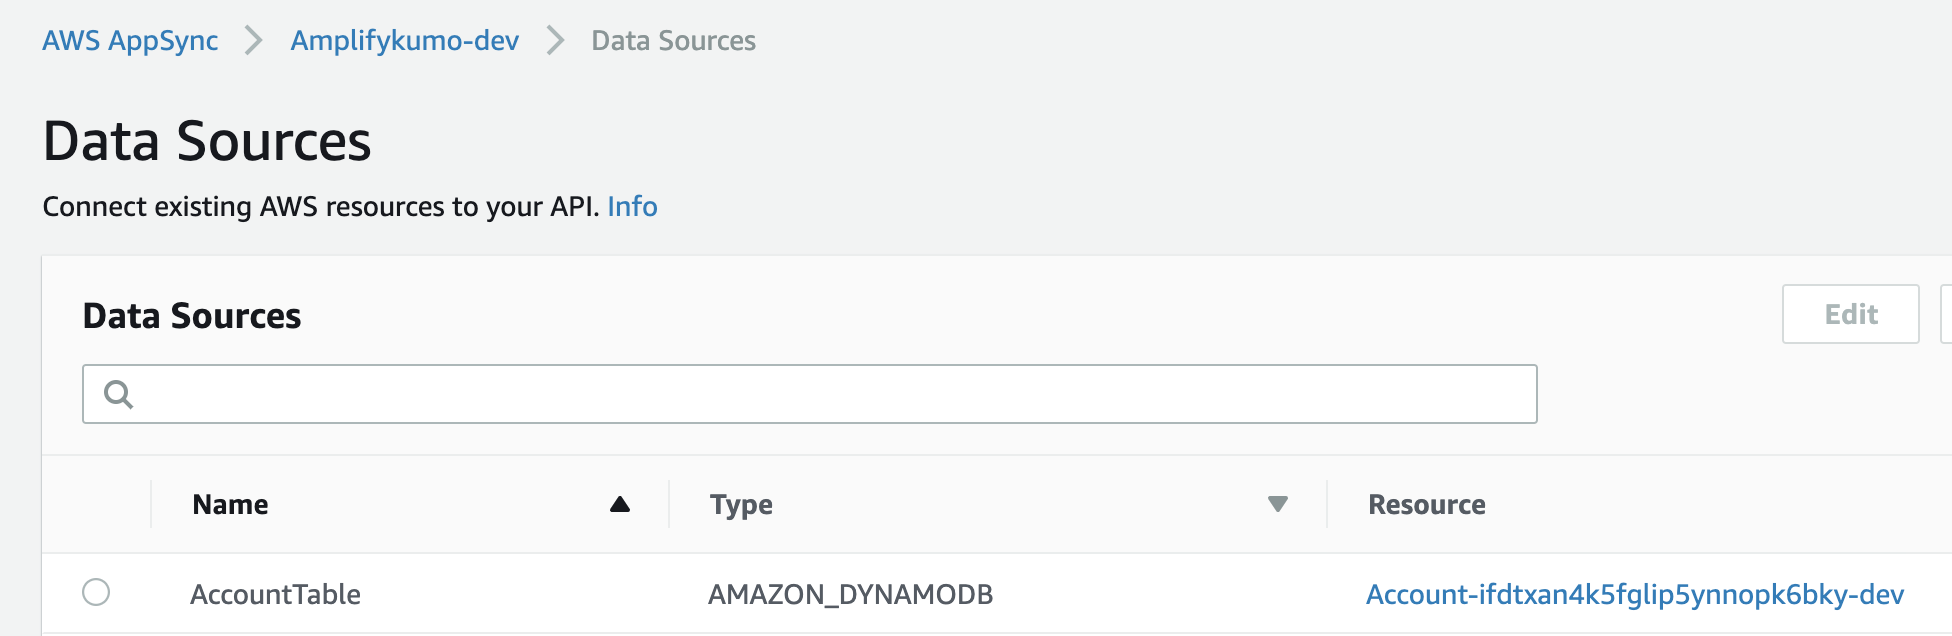
\includegraphics[width=1.0\textwidth]{50-Implementierung/AppSync-DynamoDB.png}
    \caption{Erfolg der GraphQL API Erstellung überprüfen}
    \label{fig:meine-grafik}
\end{figure}





\subsection{Implementierung Backend-Logik}
\label{ImpLambda}
Die gesamte Backend-Logik wird durch Lambda realisiert.
Mit dem Befehl \spverb+amplify add function+ startet Amplify den Prozess.
Dabei ist es im Rahmen der Bachelorarbeit ausreichend, wenn die Lambda-Funktion in regelmäßigen Abständen ausgeführt wird.
Weitere Auslöser können in Zukunft ergänzt werden.
In der Regel werden neue AWS Accounts in Abständen von zwei bis drei Wochen erstellt.
\\
\begin{lstlisting}[basicstyle=\ttfamily\small, breaklines=true , frame = single, backgroundcolor=\color{flashwhite} ]
[143302S0:amplify-kumo] master # amplify add function

Using service: Lambda, provided by: awscloudformation
Provide a friendly name for your resource to be used as
a label for this category in the project: (*@ \textrm{getallaccounts} @*)
Provide the AWS Lambda function name: (*@ \textrm{getallaccounts} @*)
Choose the function runtime that you want to use: (*@ \textrm{NodeJS} @*)
Choose the function template that you want to use:(*@ \textrm{Hello World} @*)
Do you want to access other resources created in this
project from your Lambda function? (*@ \textrm{Yes} @*)
Select the category:(*@ \textrm{storage} @*)
Do you want to invoke this function on a recurring schedule? (*@ \textrm{Yes} @*)
At which interval should the function be invoked: (*@ \textrm{Daily} @*)
Select the start time (use arrow keys):(*@ \textrm{06:35 PM} @*)

Successfully added resource getallaccounts locally.
\end{lstlisting}

\clearpage
Nachdem Amplify die Lambda-Funktion erstellt hat, kann diese direkt bearbeitet werden.
Der vollständige Code befindet sich im Anhang (Siehe Anhang \textit{\nameref{lst:LambdaCode}}).
Im Kern besteht die Lambda-Funktion aus vier Funktionen.
\\

\begin{lstlisting}[basicstyle=\ttfamily\small, breaklines=true , frame = single, backgroundcolor=\color{flashwhite} ]
getCallerIdentity()
getCrossAccountCredentials()
listAllAccounts()
writeAllDynamoDBItems()
\end{lstlisting}


Die Funktionen \spverb+getCallerIdentity()+ und \spverb+getCrossAccountCredentials()+ haben den Zweck temporären Zugriff auf den Account \spverb+Cbc-Master+ zu ermöglichen. \cite[Letzter Absatz]{Stackoverflow}
\spverb+listAllAccounts()+ liest anschließend alle Daten und \spverb+writeAllDynamoDBItems()+ schreibt diese in die DynamoDB-Tabelle.
Eine Schwierigkeit war es, eine Identität im \verb+Cbc-Master+ anzunehmen, eine weitere die korrekte Abarbeitung der Funktion sicherzustellen.
In den folgenden Abschnitten werden diese beiden Hürden genauer erläutert.

\subsubsection{Accountübergreifender Zugriff}
\label{AccountübergreifenderZugriff}
Die Lambda-Funktion befindet sich im AWS Account \verb+Cbc-Clouds-Sandbox+ und muss auf den Account \verb+Cbc-Master+ zugreifen.
Im Account \verb+Cbc-Master+ wird eine IAM-Rolle benötigt, die der Lambda-Funktion Zugriff gewährt.
Der Abschnitt  \textit{\ref{Accountstruktur} \nameref{Accountstruktur}} beschreibt den Aufbau aller Accounts der Mediengruppe RTL.
Mit IAM-Rollen können Benutzeraccounts oder AWS-Dienste temporäre Anmeldeinformationen erhalten, die Accountübergreifend funktionieren.
Dabei wird die Identität der IAM-Rolle übernommen.
Dementsprechend sind alle Operationen erlaubt, die der IAM-Rolle zugewiesen worden sind.
Damit die Lambda-Funktion also in dem Account \verb+Cbc-Master+ auf AWS Organizations zugreifen kann, benötigt die IAM-Rolle mindestens Lesezugriff auf den Dienst AWS Organizations.
AWS bietet hierfür die Berechtigung \verb+AWSOrganizationsReadOnlyAccess+.

Außerdem muss eine Vertrauensstellung hergestellt werden.
Das folgende Bild zeigt die konfigurierte Vertrauensstellung zwischen Lambda-Funktion im \verb+Cbc-Clouds-Sandbox+ und der IAM-Rolle im \verb+Cbc-Master+ Account.
Im unteren Linken Bereich bei \glqq Trusted Identities\grqq{} ist die Identität der Lambda-Funktion aus dem Account \verb+Cbc-Clouds-Sandbox+ zu sehen.
163XXXXXXXXX ist die dazugehörige AccountID.
Die IAM-Rolle hat den Namen \grqq amplify-kumo-access-role\grqq{} und besitzt einen eindeutigen Ressourcennamen (ARN).
Dieser ARN muss in der Lambda-Funktion angegeben werden. Nur so weiß die Funktion welche Identität sie übernehmen soll.

\clearpage

\begin{figure}[htbp]
    \centering
    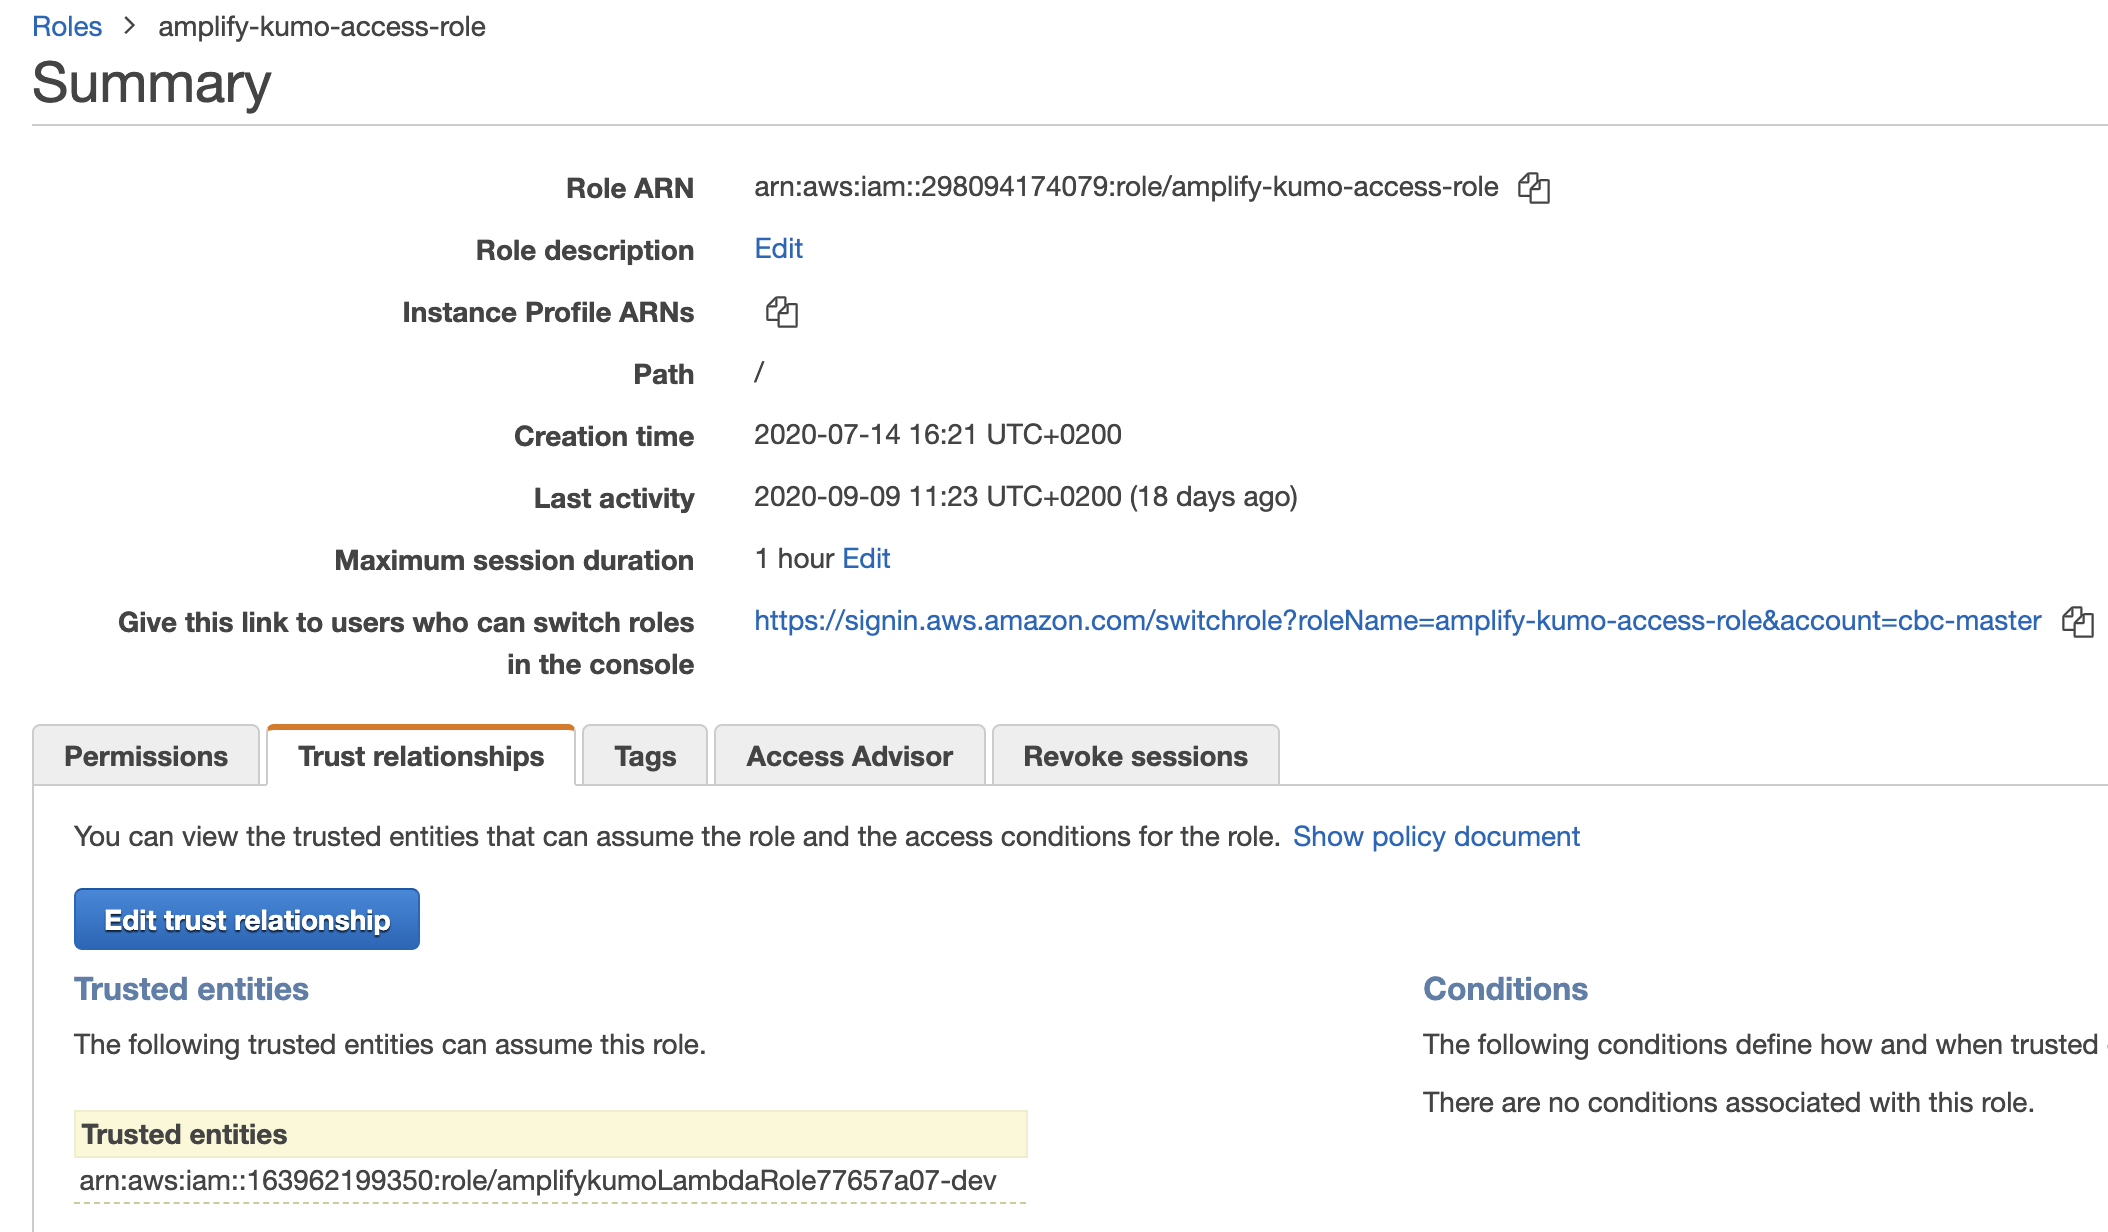
\includegraphics[width=1.0\textwidth]{50-Implementierung/IAM-Rolle.png}
    \caption{Vertrauensstellung zwischen beiden Accounts}
    \label{fig:meine-grafik}
\end{figure}


Um diesen Zugriff zu programmieren, dienen die Funktionen \verb+getCallerIdentity()+ und \verb+getCrossAccountCredentials()+.
\verb+getCallerIdentity()+ ist eine Hilfsfunktion und gibt die aktuelle Identität zurück.
So ist es leichter zu überprüfen, ob die Rolle \grqq amplify-kumo-access-role\grqq{} im \verb+Cbc-Master+ Account erfolgreich angenommen wurde.
Das eigentliche Übernehmen der IAM-Rolle erledigt \verb+getCrossAccountCredentials()+.
Es wird ein neues AWS Service-Objekt für den Dienst AWS Organizations erstellt und mithilfe der Funktion \verb+sts.assumeRole()+ ein temporärer Zugriff zum Master-Account erstellt.

Ein Service-Objekt wird benötigt, um auf Service-Funktionen zugreifen zu können.
Die meisten AWS-Dienste bieten mindestens ein passendes Service-Objekt an.
In der Lambda-Funktion muss dementsprechend ein Service-Objekt für die Dienste AWS Organizations, DynamoDB und für die Hilfsfunktion AWS STS \footnote{STS steht für Security Token Service und ermöglicht die Bereitstellung von temporären Anmeldeinformationen.} erstellt werden.
\cite{ServiceObject}

Für DynamoDB reicht etwa folgender Befehl aus, um eine passendes Service-Objekt zu erstellen.
Die Lambda-Funktion und die DynamoDB-Tabelle befinden sich im selben Account.
Auch besitzt die Lambda-Funktion bereits alle nötigen Berechtigungen, da diese durch Amplify gesetzt wurden.
\\
\begin{lstlisting}[basicstyle=\ttfamily\small, breaklines=true , frame = single, backgroundcolor=\color{flashwhite} ]
var docClient = new AWS.DynamoDB.DocumentClient
\end{lstlisting}


Für AWS Organizations müssen bei der Erstellung des Service-Objekts zusätzlich die temporären Anmeldeinformation mitgegeben werden, da sich der Dienst in einem anderen Account befindet.
Außerdem muss die Region geändert werden.
AWS Organizations ist ein Dienst, der nur in der Region \verb+us-east-1+ betrieben wird.
Für diesen Vorgang wird die Funktion \verb+getCrossAccountCredentials()+ benötigt.
Im ersten Schritt werden temporäre Anmeldeinformation abgerufen und anschließend dem Service-Objekt übergeben.

\begin{lstlisting}[basicstyle=\ttfamily\small, breaklines=true , frame = single, backgroundcolor=\color{lightgray}, caption={Neues ServiceObject mit einer anderen Identität (Datei: \textit{\nameref{lst:LambdaCode}} )} ]
var accessparams = await getCrossAccountCredentials();

const cbc_master_orgs = new AWS.Organizations({
    credentials: accessparams,
    region: 'us-east-1'
  });
\end{lstlisting}


Im Anschluss ist es möglich die Funktion \verb+listAllAccounts()+ mit einer anderen Identität auszuführen.
Dafür muss das neu erstellte ServiceObjekt übergeben werden.

\begin{lstlisting}[basicstyle=\ttfamily\small, breaklines=true , frame = single, backgroundcolor=\color{lightgray} ]
listAllAccounts(cbc_master_orgs)
\end{lstlisting}

\subsubsection{Asynchrone Verarbeitung mit NodeJS}

Alle vier Funktionen werden im Handler der Funktion nacheinander ausgeführt.
Neben den unterschiedlichen Identitäten war die Sicherstellung der asynchronen Abarbeitung ein wichtiger Aspekt bei der Programmierung.
Alle Funktionen durften nicht gleichzeitig ausgeführt werden, da sie voneinander abhängig waren.
Damit die Funktion \verb+listAllAccounts()+ erfolgreich war, musste zuvor Identität des Master-Accounts angenommen werden.
Zudem muss die Funktion \verb+writeAllDynamoDBItems()+ auf die Fertigstellung von \verb+listAllAccounts()+ warten, da sie sonst keine Daten zum Speichern hat.

Aufgrund der Abhängigkeit der Funktionen muss eine asynchrone Abarbeitung stattfinden.
Zur Option stehen dazu Callbacks, Promises oder eine Implementierung mit \verb+async/await+.
Ein Callback ist eine Funktion die an eine weitere Funktion weitergegeben wird.
So wird sichergestellt, dass die zweite Funktion erst aufgerufen wird, sobald die Erste beendet ist.
Das Problem von Callbacks ist die große Unübersichtlichkeit bei mehreren Funktionen.
Das immer tiefere verschachteln von Funktionsaufrufen wird auch als \glqq Callback-Hölle\grqq{} bezeichnet.

Promises ermöglichen dieselbe Funktionalität wie Callbacks, nur ohne die Ver­schach­telung.
\glqq Ein Promise ist ein Objekt, das die finale Beendigung einer asynchronen Operation repräsentiert.
Je nachdem, ob die Operation erfolgreich oder fehlerhaft beendet wurde, wird das Promise entsprechend gekennzeichnet. \grqq{} \cite{Promises}
Mit der Option \verb+.then()+ kann sichergestellt werden, dass die Operation beendet sein muss bevor der nächste Codeblock beginnt.

Die letzte Möglichkeit ist die Verwendung von \verb+async/await+, welche auf Promises basiert jedoch eine verständlichere Syntax ermöglicht.
Eine Funktion kann mit \verb+async+ als Asynchron deklariert werden.
Innerhalb einer asynchronen Funktion kann mit dem Operator \verb+await+ auf die Erfüllung des Promises gewartet werden.
Es ist auch möglich den Operator \verb+await+ in einer Funktion mehrmals zu verwenden.

Die Lambda-Funktion nutzt Promises und \verb+async/await+ zu einem großen Teil aus um die korrekte Abarbeitung gewährleisten zu können.
Der Event Handler wird als Asynchron deklariert und innerhalb des Handlers werden alle oben genannten Funktion nacheinander aufgerufen.

\begin{lstlisting}[basicstyle=\ttfamily\small, breaklines=true , frame = single, backgroundcolor=\color{lightgray}, caption={Beispiel zum asynchronen Funktionsaufruf (Datei: \textit{\nameref{lst:LambdaCode}})} ]
    exports.handler = async (event) => {
        [...]
      var accessparams = await getCrossAccountCredentials();
        [...]
      const all_acc = await listAllAccounts(cbc_master_orgs);
        [...]
      await writeAllDynamoDBItems([..])
    }
    \end{lstlisting}

\subsubsection{Verifizierung Lambda-Funktion}

Nach erfolgreicher Ausführung der Lambda-Funktion sollten sich Einträge in der DynamoDB-Tabelle befinden.
Zur einfachen Überprüfung kann der Dienst DynamoDB in der Webkonsole geöffnet werden.
Sind in der Tabelle Daten hinterlegt, war der Prozess erfolgreich.
Die folgende Grafik zeigt den Erfolg der Lambda-Funktion.
In der Grafik ist nur ein kleiner Ausschnitt der gespeicherten Accounts zu sehen.
Um die Eindeutigkeit sicherzustellen, wurde als ID ein MD5-Hash aus der Kombination Accountnamen und AccountID gewält.
Dies ist notwendig, da nicht ausgeschlossen werden, dass ein anderer Wert eventuell erneut auftritt.
Der Hash-Wert wird in Lambda mit dem Modul \verb+crypto+ realisiert.

\begin{figure}[htbp]
    \centering
    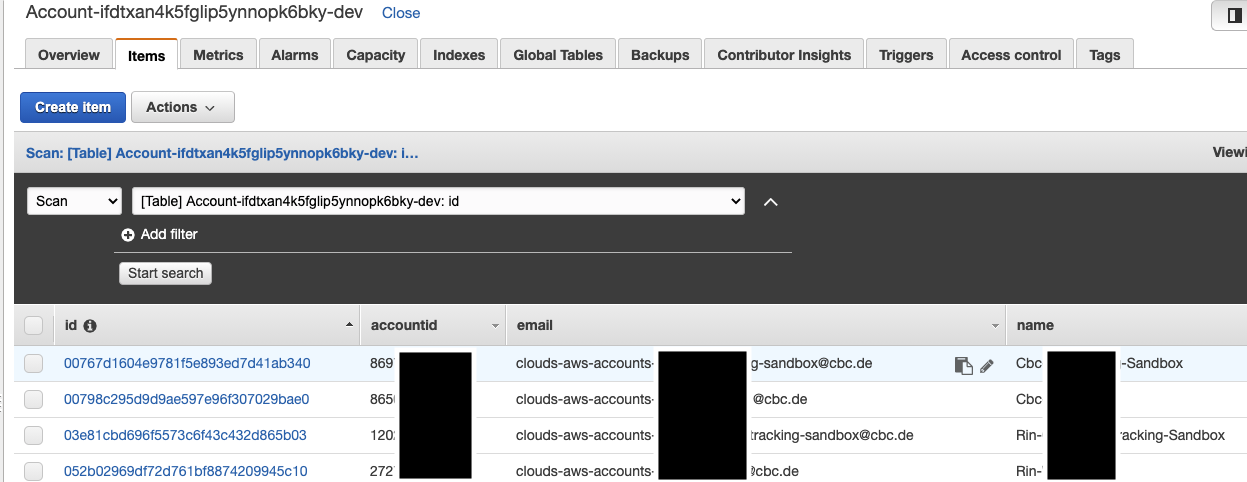
\includegraphics[width=1.0\textwidth]{50-Implementierung/DynamoWeb.png}
    \caption{Verifizierung der Lambda-Funktion}
    \label{fig:meine-grafik}
\end{figure}


\subsection{Implementierung Authentifizierung}
\label{ImpAuth}
Im Abschnitt \textit{\ref{CognitoEntscheidung} \nameref{CognitoEntscheidung}} wurde bereits erwähnt, dass Amplify in Kombination mit Cognito
alle benötigten Module für eine vollständige Authentifizierung beinhaltet.
Um die erforderliche Komponente hinzuzufügen, muss der Befehl \verb+amplify add auth+ ausgeführt werden.
Im darauffolgenden Assistenten kann die gewünschte Option zur Anmeldung gewählt werden.
Nach dem Befehl \verb+amplify push+ wird ein Cognito User Pool inklusive App Clients erstellt.
Über die Webkonsole besteht im Anschluss die Option MFA zu aktivieren.

Für die Einbindung in das React-Frontend bietet das Amplify-Framework die Komponente \verb+withAuthenticator+ an.
Diese muss um die Hauptkomponente umhüllt werden.
Dafür wird beim Exportieren der Hauptkomponente \verb+withAuthenticator+ mitangegeben. \cite{ImpAuth}
Die React-Komponente \verb+AWSAccountListsMaterial+ beinhaltet den Code zum Abfragen der Daten aus der DynamoDB-Tabelle und zum Rendern der Übersicht.

Mehr Details zu der Komponente befinden sich im Abschnitt \textit{\ref{ReactFrontend} \nameref{ReactFrontend}}.
\\
\begin{lstlisting}[basicstyle=\ttfamily\small, breaklines=true , frame = single, backgroundcolor=\color{flashwhite},caption={Auszug aus React-Frontend (Datei: \textit{\nameref{lst:React AccountList}} )} ]
import { withAuthenticator, AmplifySignOut } from "@aws-amplify/ui-react";

class AWSAccountListsMaterial extends React.Component {
[...]
}
export default withAuthenticator(AWSAccountListsMaterial, true)
    \end{lstlisting}



Startet man den lokalen Webserver im Anschluss und ruft die Anwendung auf, erscheint eine voll funktionsfähige Login-Maske.
Diese Ansicht lässt sich auf Wunsch auch anpassen.
Damit nicht jede Person einen Account erstellen kann, ist die Option \glqq Allow users to sign themselves up\grqq{} in der Webkonsole deaktiviert und die Option \glqq Only allow administrators to create users\grqq{} aktiviert worden.
Wird über \glqq Create Account\grqq{} versucht einen neuen Benutzer zu erstellen, erscheint die Meldung \glqq SignUp is not permitted for this user pool\grqq{}.
Ohne Cognito und Amplify wäre die Implementierung einer sicheren und funktionierenden Authentifizierungsmethode deutlich aufwändiger.
Dank der vorgefertigten Module ist es mit Amplify jedoch schnell umsetzbar.

\begin{figure}[htbp]
    \centering
    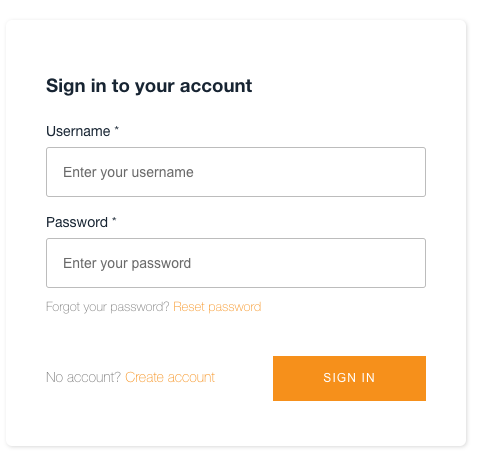
\includegraphics[width=0.5\textwidth]{50-Implementierung/Login.png}
    \caption{Login-Maske mit Amplify und Cognito}
    \label{fig:meine-grafik}
\end{figure}


Da Cognito erfolgreich implementiert wurde, kann die Authentifizierung in der API geändert werden.
Mit dem Befehl \spverb+amplify update api+ kann jetzt der Cognito Benutzerpool ausgewählt werden.
Im Anschluss kann die Änderung mit \spverb+amplify publish+ veröffentlicht werden.


\subsubsection{Anmeldung über AzureAD}

Wie im Abschnitt \textit{\ref{Authentifizierung} \nameref{Authentifizierung}} bereits erwähnt, wäre es wünschenswert die Anmeldung mit Unternehmensidentitäten zu ermöglichen.
Die Mediengruppe RTL nutzt hierfür den Dienst Azure Active Directory.
Mittlerweile sind einige Anbindungen als SSO über AzureAD verfügbar.
Die Anmeldung zu allen drei Cloud Providern erfolgt etwa über die gemeinsame Identität des Unternehmens.

Cognito bietet eine Unterstützung mit Unternehmens-Identitätsanbietern über SAML an.
Dafür müssen Konfigurationen in AzureAD und AWS Cognito getätigt werden.
Während des Vorgangs ist schließlich die Entscheidung gefallen, dass es keine geeignete Implementierung in Zusammenspiel mit Amplify gibt.
Im Internet existieren mehrere Anleitungen zur Verbindung von AzureAD mit Cognito, jedoch ohne Amplify.
Der Cognito Dienst wurde dabei mit einer \glqq Azure Enterprise Application\grqq{} verknüpft.
Bei \glqq Azure Enterprise Application\grqq{} handelt es sich um einen Dienst, der zur Verwaltung von Identitäten genutzt wird.
Nach der Einrichtung sind leider Fehlermeldungen aufgetreten.
Das Ergebnis einer Recherche zeigte, dass Amplify für diese spezielle Anbindung nicht optimiert ist.
Der SSO Authentifizierungsweg muss in das Frontend eingebaut werden.
Für diesen Prozess existieren im Internet mehrere Dokumentationen für Android oder iOS Apps.
Für React oder ein anderes JavaScript-Framework scheint die Integration komplexer zu sein.
Auf der Website \textit{\href{https://dunlop.geek.nz/aws-cognito-azure-ad-react-amplify/}{dunlop.geek.nz}} wird ein Lösungsvorschlag angeboten, der jedoch im Rahmen dieser Bachelorarbeit nicht umgesetzt wird.
Laut der Anleitung ist es notwendig mehrere Stellen im Frontend stark zu bearbeiten und einen großen Teil der Authentifizierung manuell zu erstellen.
Zudem ist es laut Autor notwendig die Datei \verb+aws-exports.js+ zu bearbeiten.
In der Datei selbst wird davor explizit gewarnt.

\begin{lstlisting}[basicstyle=\ttfamily\small, breaklines=true , frame = single, backgroundcolor=\color{flashwhite}, caption={Auszug aws-exports.js} ]
// WARNING: DO NOT EDIT. This file is automatically generated by AWS Amplify. It will be overwritten.
\end{lstlisting}

Aufgrund des hohen Aufwands und der nicht zufriedenstellenden Lösung wird die Anwendung vorerst ohne eine Anbindung auskommen.
Mitarbeiter, die Zugang benötigten, müssen sich über einen separaten Account anmelden.
Falls in Zukunft eine bessere Option zur Verfügung steht, kann sie jederzeit hinzugefügt werden, ohne das bestehende System zu beeinträchtigen.


\subsection{Implementierung Frontend und Hosting}

\subsubsection{Programmierung React-Frontend}
\label{ReactFrontend}
Im letzten Schritt der Implementierung muss das Frontend konfiguriert werden und die Anwendung veröffentlicht werden.
Bisher verfügt das Frontend über Authentifizierung, und dank der Lambda-Funktion sind Informationen in der DynamoDB-Tabelle verfügbar.
Nun müssen mit React und AppSync eine Abfrage der Daten stattfinden.
Im Anschluss werden diese Daten visualisiert.

Um erste Erfahrungen mit React zu sammeln, wurde eine Komponente zur Begrüßung erstellt.
Die React-Komponente \verb+<Greeting>+ gibt zwei simple HTML Elemente mit einem definierten Text zurück.
Als Nächstes wurde die React-Komponente \verb+<AWSAccountListsMaterial>+ erzeugt, die für die restliche Logik zuständig ist.

Zuallererst wird eine Query benötigt, die alle Daten der Tabelle abfragt und in der Komponente genutzt werden kann.
In der Query werden alle Felder ausgewählt, die im Schema angegeben wurden, da alle auch benötigt werden.
Wie zuvor erwähnt wurde, ist es ebenfalls möglich auch nur einen Teil der Felder abzufragen und so ein Over-fetching zu vermeiden.

\begin{lstlisting}[basicstyle=\ttfamily\small, breaklines=true , frame = single, backgroundcolor=\color{flashwhite},caption={Query zum Accountaufruf (Datei: \textit{\nameref{lst:React AccountList}} )} ]
// GraphQL Query to get all data
 const listAllAccounts = `query listAllAccounts {
    listAccounts (limit: 300) {
      items{
        id
        accountid
        num
        name
        email
        status
        }
      } }`;
    \end{lstlisting}



Auch hier muss eine asynchrone Abarbeitung sichergestellt werden.
Die Daten müssen zur Verfügung stehen, bevor sie gerendert werden können.
React bietet dazu die Funktion \verb+componentDidMount()+ an, die exakt für diesen Anwendungsfall existiert. \cite{ReactComp}
Innerhalb der Funktion \verb+componentDidMount()+ wird eine weitere Funktion \verb+queryAccounts()+ gestartet.
Diese Funktion führt mithilfe von AppSync die Query aus und speichert sie in die State Variable.\cite{AmplifyAPI}
State kann alle internen Daten einer Komponente beinhalten.
Wird die State Variable mithilfe von \verb+setState()+ geändert, ruft React automatisch die Renderfunktion erneut auf und aktualisiert die Seite.

\begin{lstlisting}[basicstyle=\ttfamily\small, breaklines=true , frame = single, backgroundcolor=\color{flashwhite},caption={Abruf der Daten und Speicherung in State Variable (Datei: \textit{\nameref{lst:React AccountList}} )} ]
queryAccounts = async() => {
    try {
      const result = await API.graphql(graphqlOperation(listAllAccounts))
      const result_json = Object.values(result)
      const result_optimized = result_json[0].listAccounts.items
      // this will re render the view with new data
      this.setState({
        AccountList:result_optimized,})
    } catch (err) {
      console.log(err);
    }}
\end{lstlisting}


Im letzten Schritt müssen die Information aus der State Variable im Frontend angezeigt werden.
Hierfür eignet sich eine tabellarische Ansicht am meisten.
Zuerst wurde mit JSX ein HTML \verb+<table>+ Element erstellt und die einzelnen Daten korrekt hinzugefügt.
Da hierbei jedoch weitere Funktionalitäten manuell entwickelt werden müssten, wurde letztendlich die frei zugängliche Komponente \glqq material-table\grqq{} genutzt.
Diese Komponente ermöglicht das Erstellen einer übersichtlichen Tabelle mit den wichtigsten Features, etwa einer Suche oder einer Sortierfunktion.
Zudem ist nahezu jeder Aspekt frei konfigurierbar, etwa die Anzahl an Elementen pro Seite.\cite{MaterialTable}
Innerhalb der \verb+<AWSAccountListsMaterial>+ wird also die externe Komponente \verb+<MaterialTable>+ eingebeut.
Hier werden die Spalten konfiguriert, sowie dem Feld \glqq data\grqq{} die Daten aus der State Variable übergeben.

\begin{lstlisting}[basicstyle=\ttfamily\small, breaklines=true , frame = single, backgroundcolor=\color{flashwhite} ]
<MaterialTable
[...]
columns={[
  { title: 'Nummer', field: 'num', defaultSort: "asc", width: '6%' },
  { title: 'Name', field: 'name', width: '30%' },
  { title: 'Account ID', field: 'accountid' },
  { title: 'Email', field: 'email', width: '50%', align: "center" },
  { title: 'Status', field: 'status', sorting:false, width: '6%'}
 ]}
          data={this.state.AccountList}
/>
    \end{lstlisting}


 Das folgende Bild zeigt das Ergebnis nach der Implementierung des Codes.
 Sollte aus irgendwelchen Gründen der Abruf der Daten fehlschlagen, zeigt React nur eine leere Tabelle an.
 Zum gegebenen Zeitpunkt existierten 162 Einträge, wovon jeweils 30 pro Seite angezeigt wurden.
 Die Implementierung aller Dienste wurde erfolgreich durchgeführt.

 \begin{figure}[htbp]
    \centering
    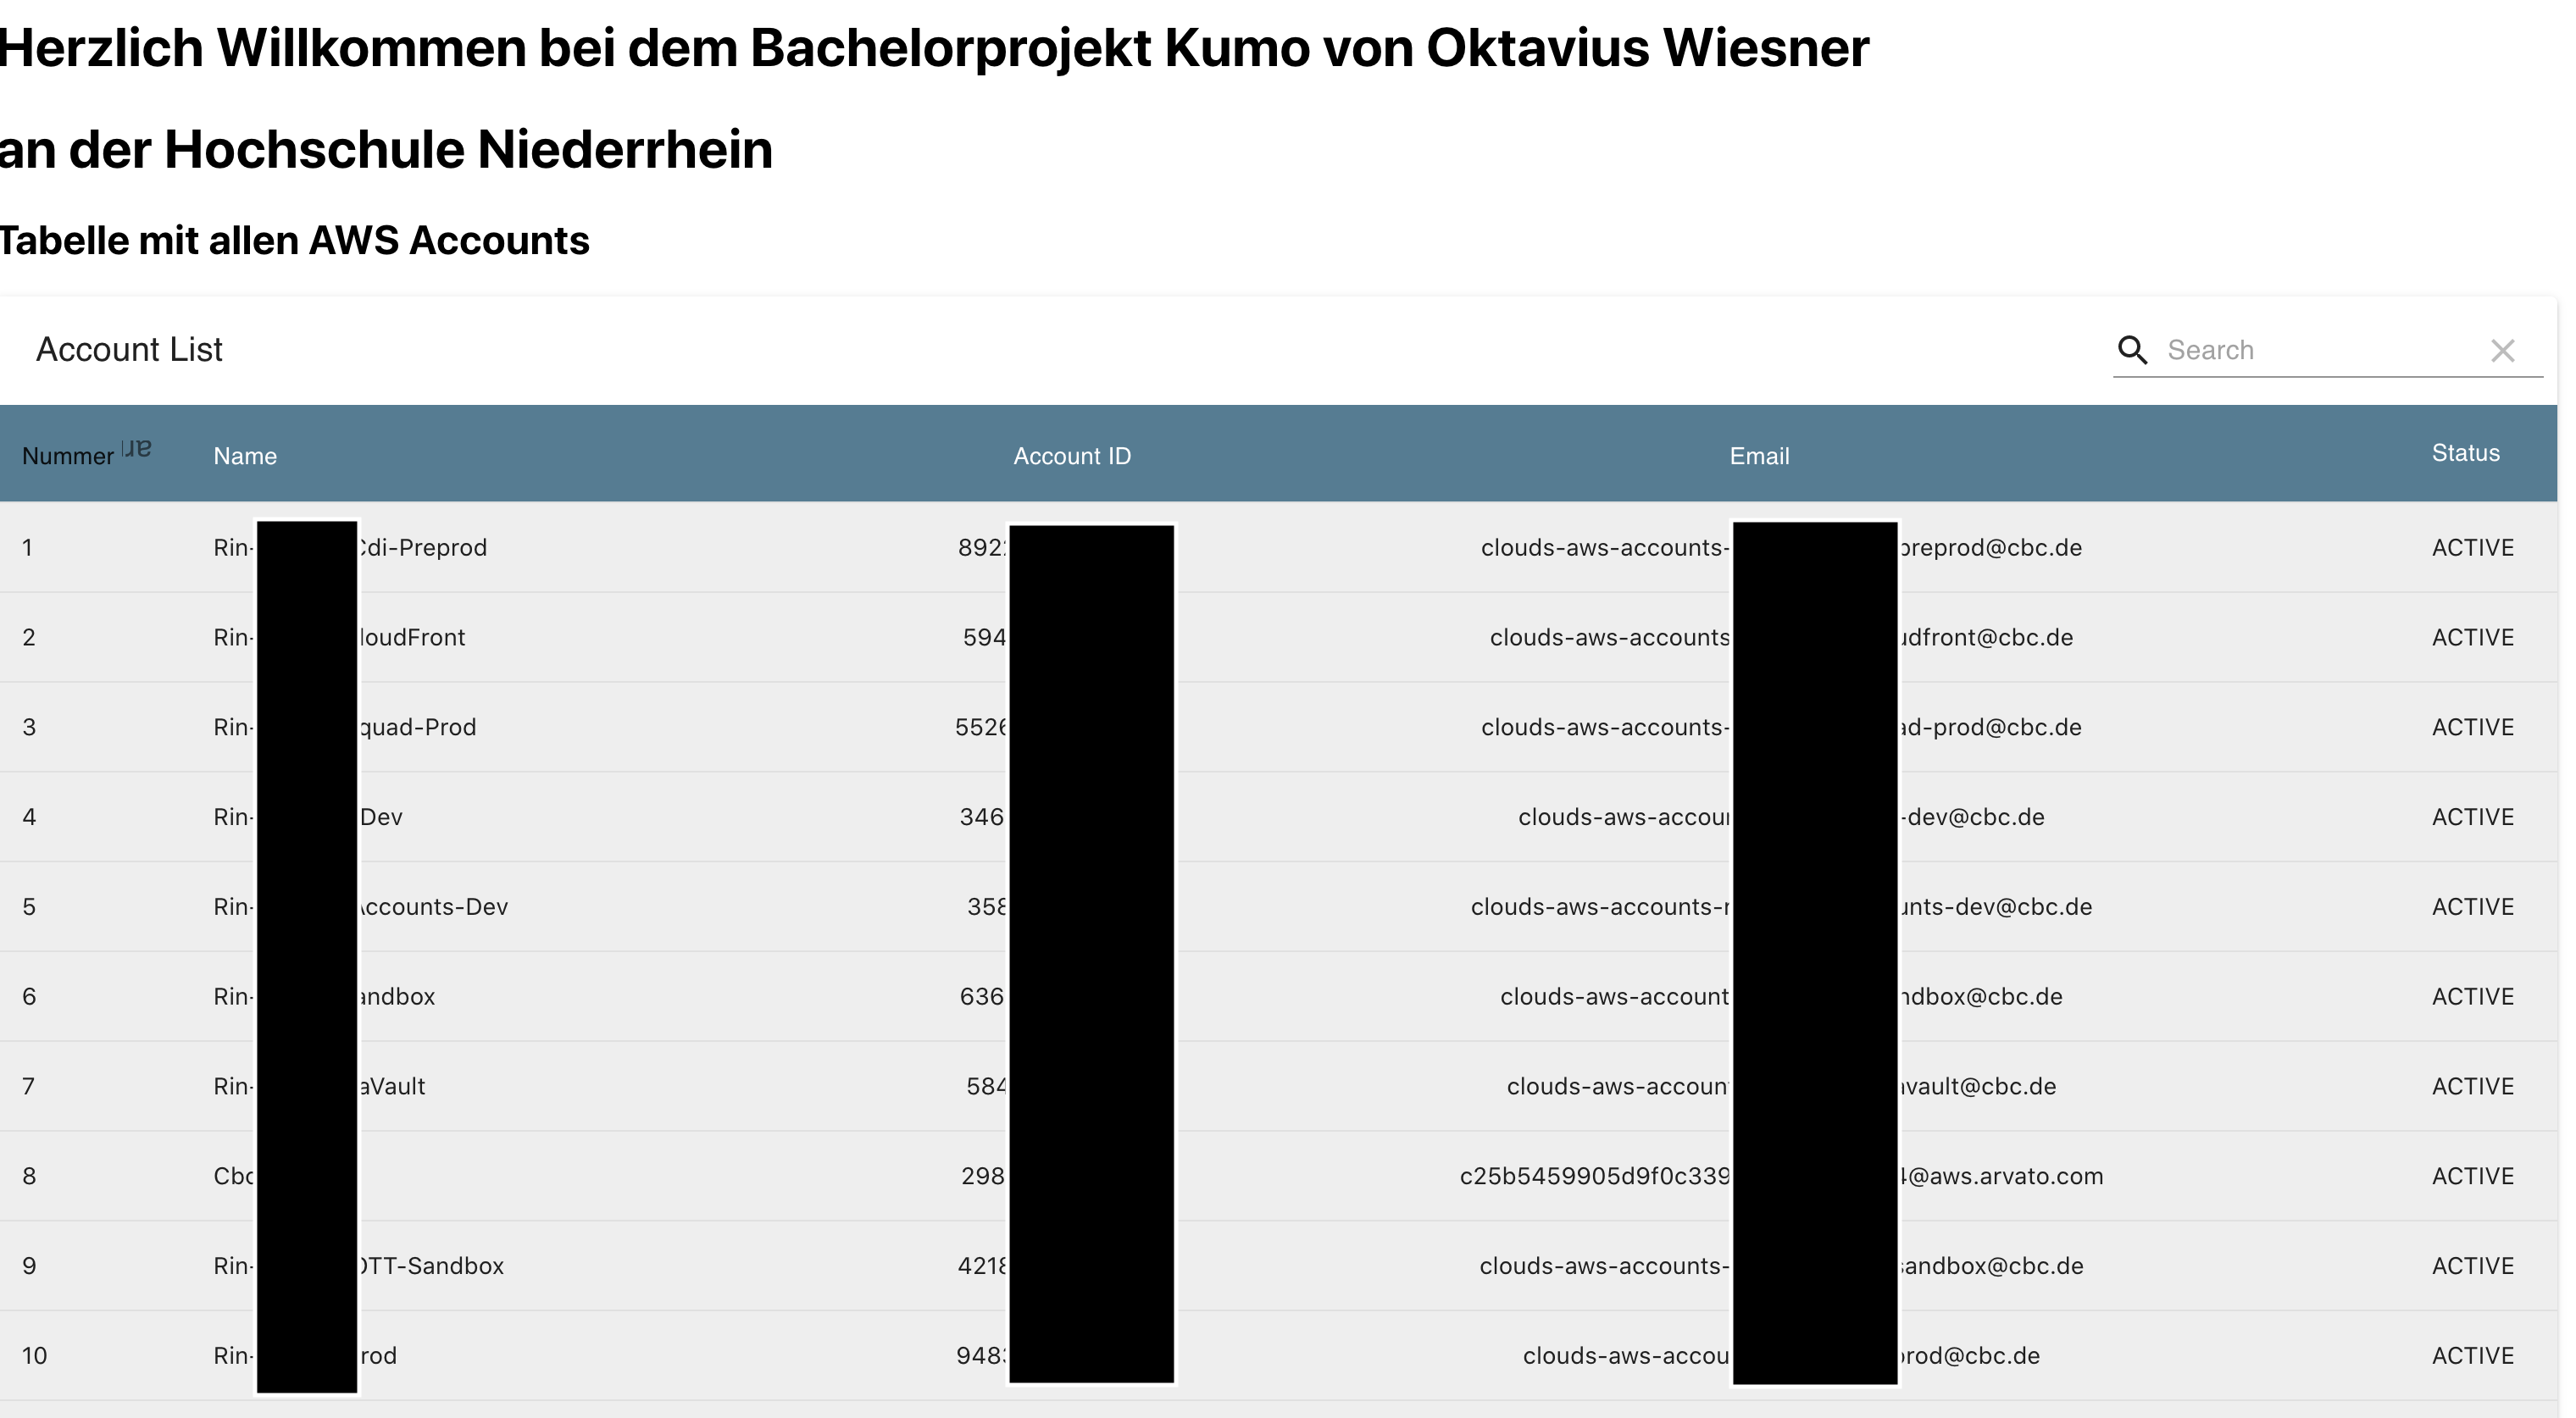
\includegraphics[width=1.0\textwidth]{50-Implementierung/Webanwendung.png}
    \caption{Fertiggestellte Website mit Daten}
    \label{fig:FertigSeite}
\end{figure}

\subsubsection{Hosting}

Da alle Komponenten erfolgreich implementiert worden sind und die Webanwendung alle geforderten Aufgaben erfüllt, kann sie veröffentlicht werden.
Mithilfe von \verb+amplify add hosting+ kann die Webanwendung bei Amazon gehosted werden.
In diesem Schritt kann Amplify zudem eine Integration mit GitHub übernehmen.
Es wird ein bestimmtes Repository mit Amplify verknüpft.
Sobald neuer Code in das Repository hochgeladen wird, startet Amplify ein automatisches Deployment mit diesen Änderungen.
Werden mehrere Branches mit unterschiedlichen Umgebungen genutzt, können diese ebenfalls seperat hinzugefügt werden.
Nach Fertigstellung gibt Amplify eine URL zurück über die die Anwendung aufgerufen werden kann.
\\
\begin{lstlisting}[basicstyle=\ttfamily\small, breaklines=true , frame = single, backgroundcolor=\color{flashwhite} ]
[143302S0:amplify-kumo] master # amplify add hosting
Select the plugin module to execute Hosting with Amplify Console
(*@ \textrm{Managed hosting with custom domains, Continuous deployment} @*)

Choose a type Continuous deployment (*@ \textrm{Git-based deployments} @*)
Continuous deployment is configured in the Amplify Console.
Please hit enter once you connect your repository
[...]
Amplify hosting urls:
FrontEnd Env       Domain
dev                https://dev.drjgagjbys8gs.amplifyapp.com

    \end{lstlisting}

Auf Wunsch kann eine eigene Domäne hinzugefügt werden, sodass die \spverb+.amplifyapp.com+ Domäne nicht zwingend genutzt werden muss.
In dem Account \spverb+Cbc-Clouds-Sandbox+ ist bereits die Domäne \spverb+sandboxzone.aws-cbc.cloud+ registriert.
Somit kann direkt über dem Menüpunkt \glqq Domain Management\grqq{} eine Subdomäne für die Webanwendung konfiguriert werden.
Falls die Domain über AWS registirert wurde, kümmert sich Amplify automatisch um das Erstellen des SSL-Zertifikates\footnote{SSL steht für Secure Sockets Layer und ist ein Protokoll zum eindeutigen Identitätsnachweis. Heutzutage werden SSL-Zertifikate mit TLS(Transport Layer Security) verschlüsselt. Ein Zertifikat enthählt viele Informationen, etwa den Namen des Ausstellers, und wird von einer Zertifizierungsstelle ausgestellt.} und Setzen des CNAMEs.


\begin{figure}[htbp]
    \centering
    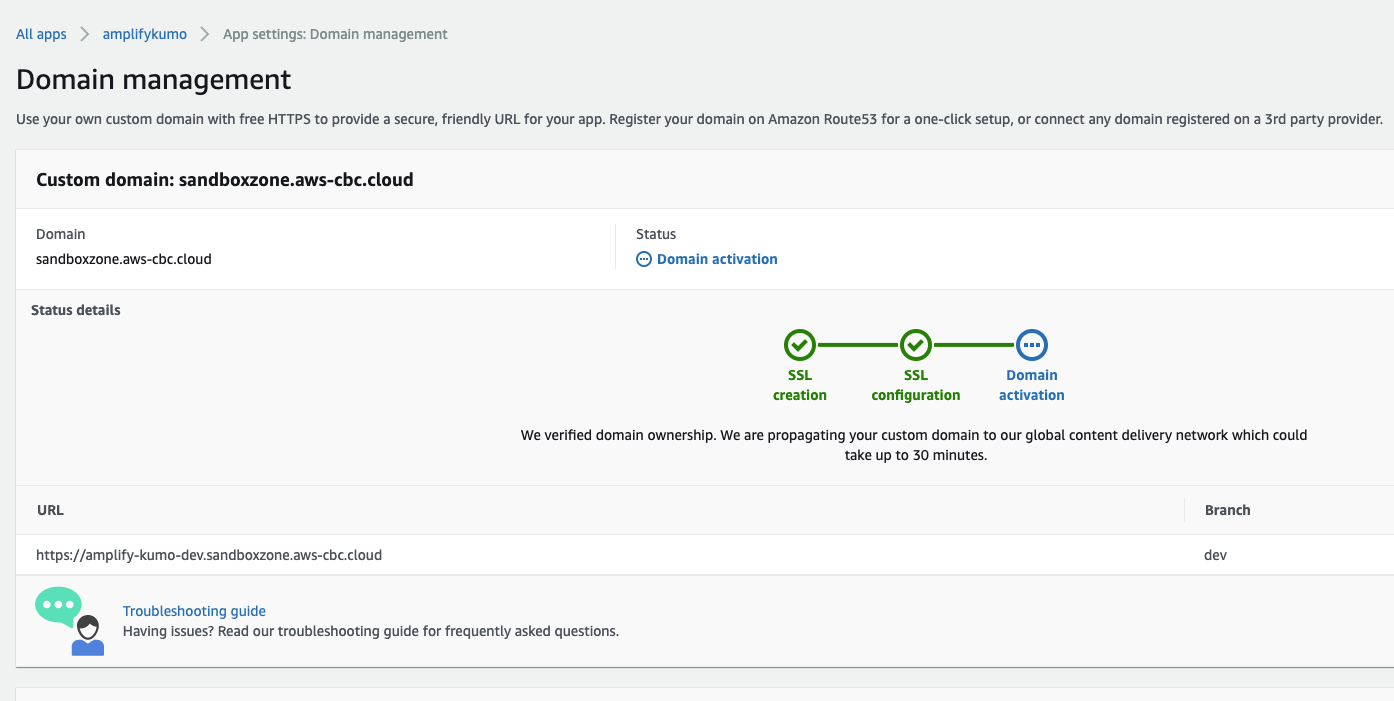
\includegraphics[width=1.0\textwidth]{50-Implementierung/SSL.png}
    \caption{Konfigurieren einer eigenen Domain}
    \label{fig:meine-grafik}
\end{figure}

Sobald der DNS Eintrag verfügbar ist, kann die Webanwendung unter folgender Adresse aufgerufen werden.
Für jede Entwicklungsumgebung lässt sich eine eigene Subdomain konfigurieren.
\\
\begin{lstlisting}[basicstyle=\ttfamily\small, breaklines=true , frame = single, backgroundcolor=\color{flashwhite} ]
https://amplify-kumo-dev.sandboxzone.aws-cbc.cloud
\end{lstlisting}
